\documentclass{standalone}
\usepackage{tikz}
\begin{document}
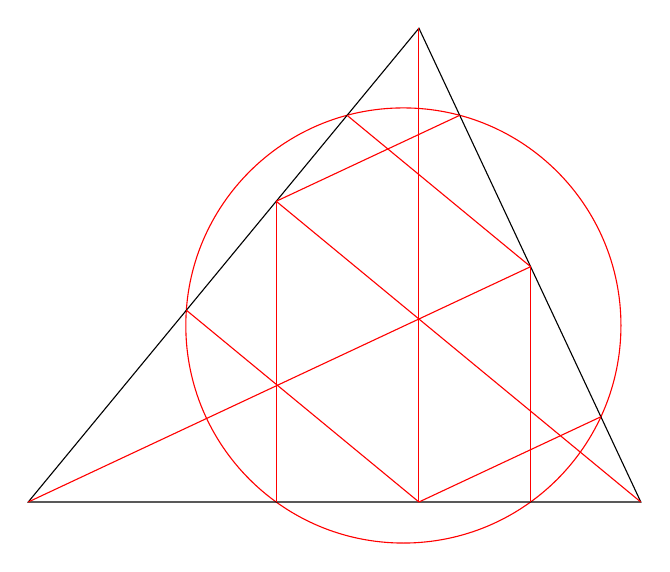
\begin{tikzpicture}[x=1pt,y=1pt]
\draw[red] (170.47,-144.52) circle (78.62);
\draw (256.27,-208.31) -- (176.09,-37.11) -- (34.91,-208.31) -- cycle;
\draw[red] (176.09,-37.11) -- (176.09,-208.31);
\draw[red] (34.91,-208.31) -- (216.45,-123.27);
\draw[red] (216.44,-123.27) -- (150.12,-68.58);
\draw[red] (216.44,-123.27) -- (216.44,-208.31);
\draw[red] (176.09,-208.31) -- (241.84,-177.51);
\draw[red] (176.09,-208.31) -- (92.06,-139.01);
\draw[red] (124.52,-99.64) -- (190.83,-68.58);
\draw[red] (124.52,-99.64) -- (124.52,-208.30);
\draw[red] (256.26,-208.31) -- (124.52,-99.64);
\end{tikzpicture}
\end{document}
